
\begin{figure*}
  \centering
  \begin{subfigure}[b]{0.15\textwidth}
    \begin{tikzpicture}[
        spy using outlines={%
          rectangle,magnification=3,size=\textwidth,
          every spy on node/.append style={transparentwindow}
        }
      ]
      \node (figA) at (0.0,0.0) {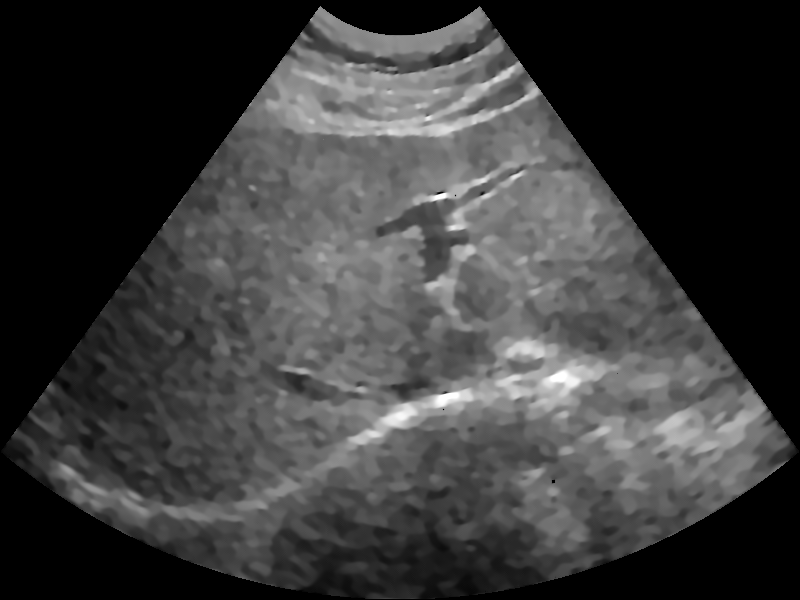
\includegraphics[width=\textwidth, trim={4cm 4cm 4cm 0cm}, clip]{figures/liver1_osrad.png}};
      \spy on (0.15, 0.0) in node [redwindow, anchor=north] at ($(figA.south)$);
    \end{tikzpicture}
    \caption{OSRAD}
  \end{subfigure}%
  \begin{subfigure}[b]{0.15\textwidth}
    \begin{tikzpicture}[
        spy using outlines={%
          rectangle, magnification=3,size=\textwidth,
          every spy on node/.append style={transparentwindow}
        }
      ]
      \node (figA) at (0.0,0.0) {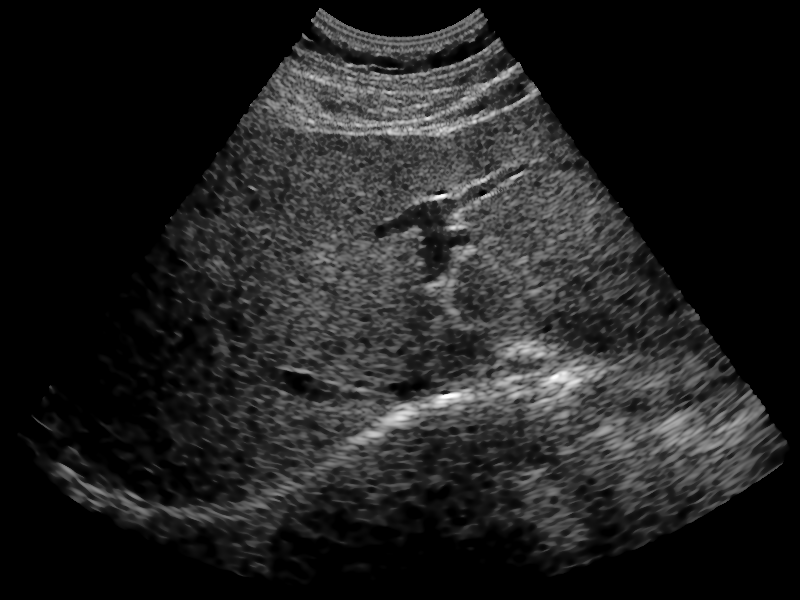
\includegraphics[width=\textwidth, trim={4cm 4cm 4cm 0cm}, clip]{figures/liver1_admss.png}};
      \spy on (0.15, 0.0) in node [redwindow, anchor=north] at ($(figA.south)$);
    \end{tikzpicture}
    \caption{ADMSS}
  \end{subfigure}%
  \begin{subfigure}[b]{0.15\textwidth}
    \begin{tikzpicture}[
        spy using outlines={%
          rectangle, magnification=3,size=\textwidth,
          every spy on node/.append style={transparentwindow}
        }
      ]
      \node (figA) at (0.0,0.0) {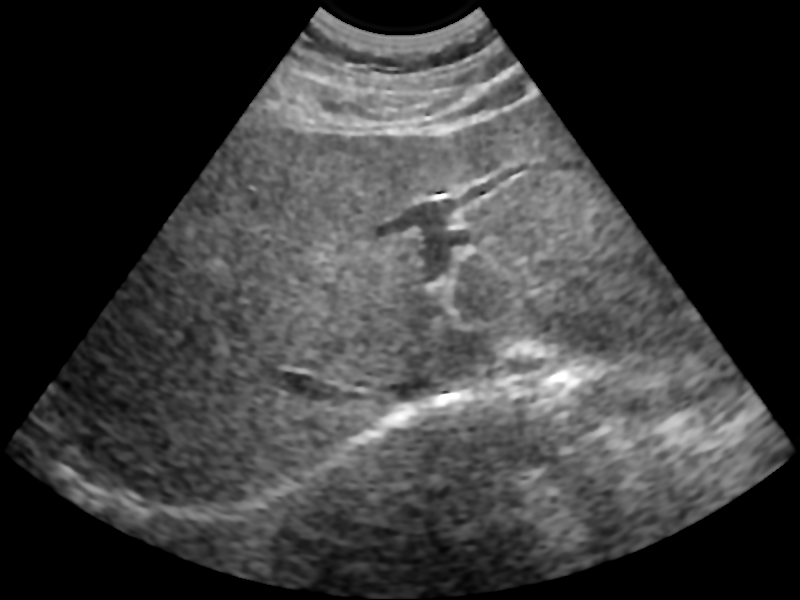
\includegraphics[width=\textwidth, trim={4cm 4cm 4cm 0cm}, clip]{figures/liver1_lpndsf.png}};
      \spy on (0.15, 0.0) in node [redwindow, anchor=north] at ($(figA.south)$);
    \end{tikzpicture}
    \caption{LPNDSF}
  \end{subfigure}%
  \begin{subfigure}[b]{0.15\textwidth}
    \begin{tikzpicture}[
        spy using outlines={%
          rectangle,magnification=3,size=\textwidth,
          every spy on node/.append style={transparentwindow}
        }
      ]
      \node (figA) at (0.0,0.0) {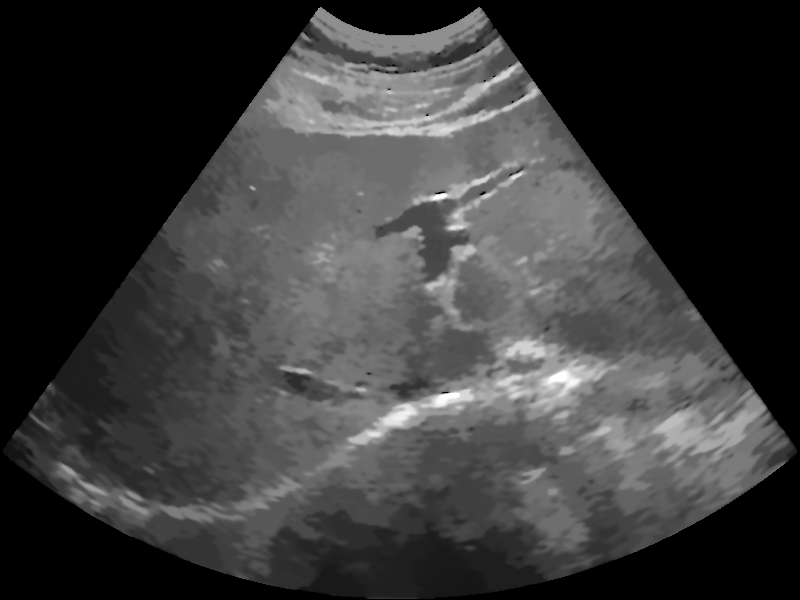
\includegraphics[width=\textwidth, trim={4cm 4cm 4cm 0cm}, clip]{figures/liver1_mnlm.png}};
      \spy on (0.15, 0.0) in node [redwindow, anchor=north] at ($(figA.south)$);
    \end{tikzpicture}
    \caption{MNLM}
  \end{subfigure}%
  \begin{subfigure}[b]{0.15\textwidth}
    \begin{tikzpicture}[
        spy using outlines={%
          rectangle,magnification=3,size=\textwidth,
          every spy on node/.append style={transparentwindow}
        }
      ]
      \node (figA) at (0.0,0.0) {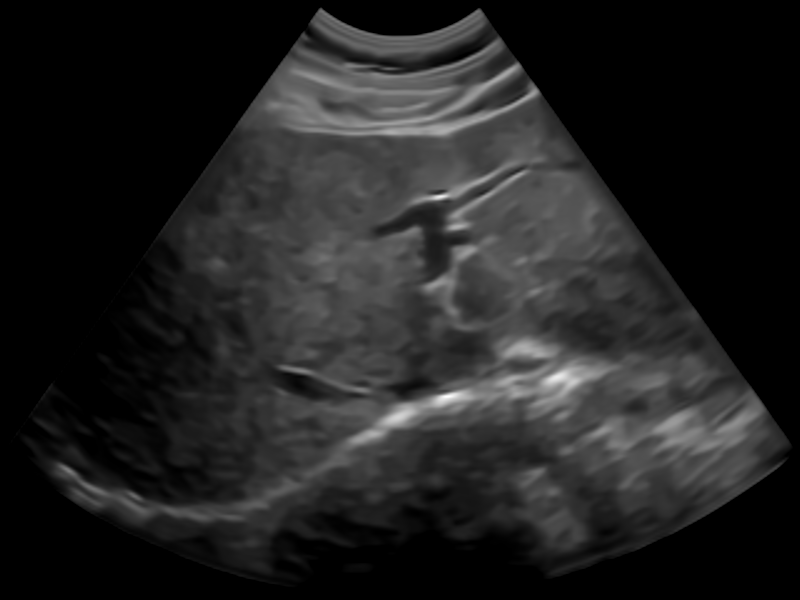
\includegraphics[width=\textwidth, trim={4cm 4cm 4cm 0cm}, clip]{figures/liver1_nllr.png}};
      \spy on (0.15, 0.0) in node [redwindow, anchor=north] at ($(figA.south)$);
    \end{tikzpicture}
    \caption{NLLR}
  \end{subfigure}%
  \begin{subfigure}[b]{0.15\textwidth}
    \begin{tikzpicture}[
        spy using outlines={%
          rectangle,magnification=3,size=\textwidth,
          every spy on node/.append style={transparentwindow}
        }
      ]
      \node (figA) at (0.0,0.0) {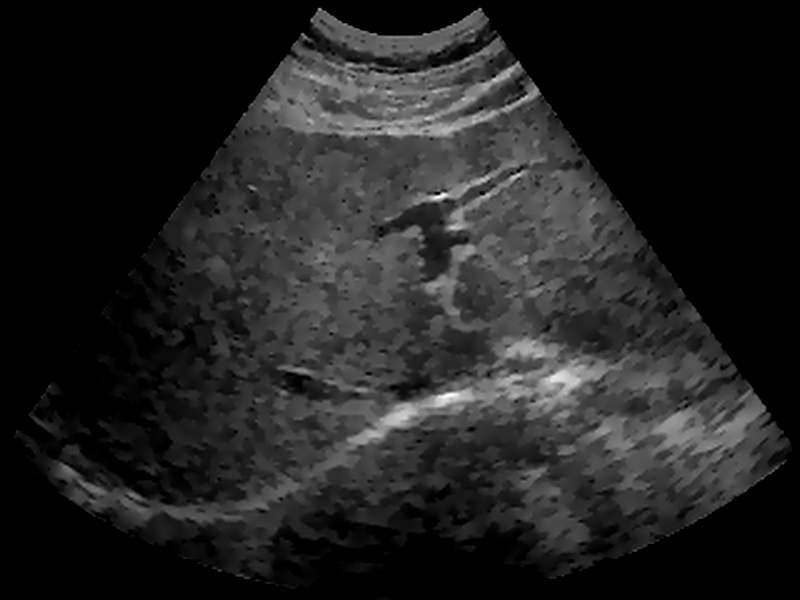
\includegraphics[width=\textwidth, trim={4cm 4cm 4cm 0cm}, clip]{figures/liver1_pfdtv.png}};
      \spy on (0.15, 0.0) in node [redwindow, anchor=north] at ($(figA.south)$);
    \end{tikzpicture}
    \caption{PFDTV}
  \end{subfigure}\\
  \begin{subfigure}[b]{0.15\textwidth}
    \begin{tikzpicture}[
        spy using outlines={%
          rectangle,magnification=3,size=\textwidth,
          every spy on node/.append style={transparentwindow}
        }
      ]
      \node (figA) at (0.0,0.0) {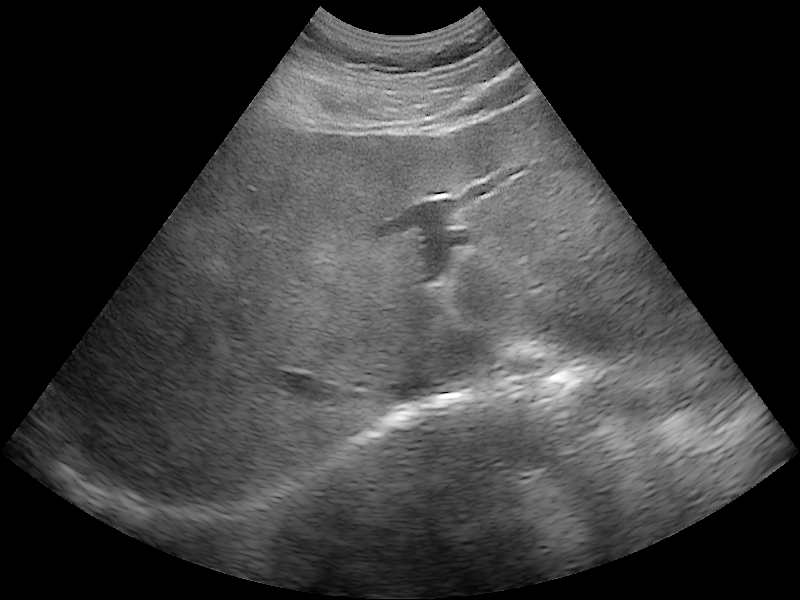
\includegraphics[width=\textwidth, trim={4cm 4cm 4cm 0cm}, clip]{figures/liver1_clpdQ.png}};
      \spy on (0.15, 0.0) in node [redwindow, anchor=north] at ($(figA.south)$);
    \end{tikzpicture}
    \caption{CLPD-SSNR}
  \end{subfigure}%
  \begin{subfigure}[b]{0.15\textwidth}
    \begin{tikzpicture}[
        spy using outlines={%
          rectangle,magnification=3,size=\textwidth,
          every spy on node/.append style={transparentwindow}
        }
      ]
      \node (figA) at (0.0,0.0) {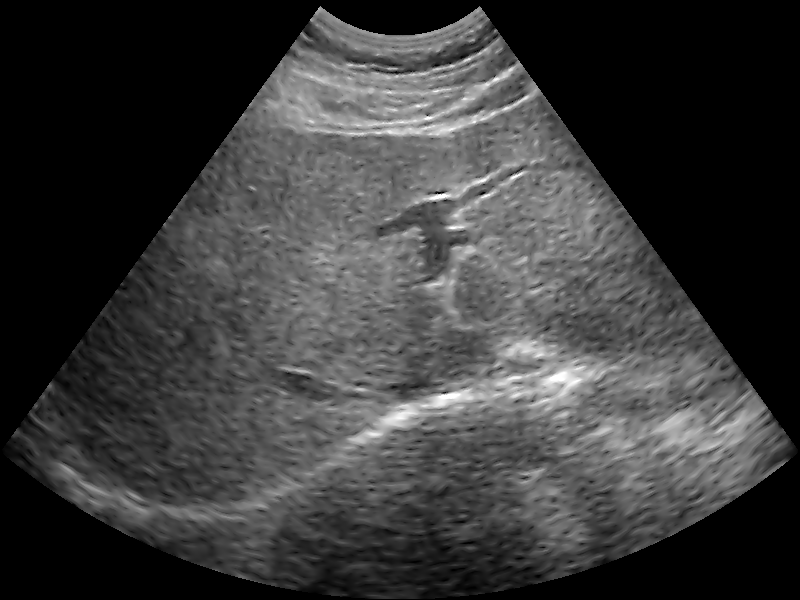
\includegraphics[width=\textwidth, trim={4cm 4cm 4cm 0cm}, clip]{figures/liver1_clpda.png}};
      \spy on (0.15, 0.0) in node [redwindow, anchor=north] at ($(figA.south)$);
    \end{tikzpicture}
    \caption{CLPD-A}
  \end{subfigure}%
  \begin{subfigure}[b]{0.15\textwidth}
    \begin{tikzpicture}[
        spy using outlines={%
          rectangle,magnification=3,size=\textwidth,
          every spy on node/.append style={transparentwindow}
        }
      ]
      \node (figA) at (0.0,0.0) {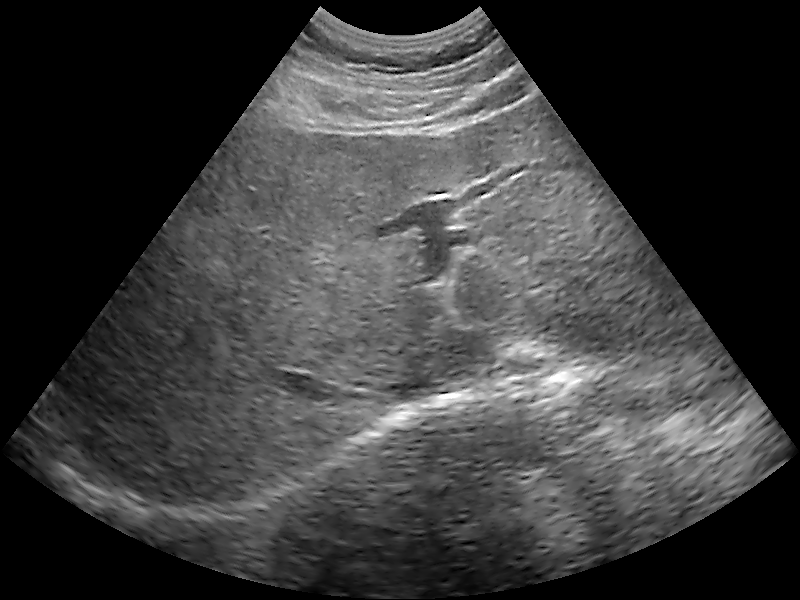
\includegraphics[width=\textwidth, trim={4cm 4cm 4cm 0cm}, clip]{figures/liver1_clpdb.png}};
      \spy on (0.15, 0.0) in node [redwindow, anchor=north] at ($(figA.south)$);
    \end{tikzpicture}
    \caption{CLPD-B}
  \end{subfigure}%
  \begin{subfigure}[b]{0.15\textwidth}
    \begin{tikzpicture}[
        spy using outlines={%
          rectangle,magnification=3,size=\textwidth,
          every spy on node/.append style={transparentwindow}
        }
      ]
      \node (figA) at (0.0,0.0) {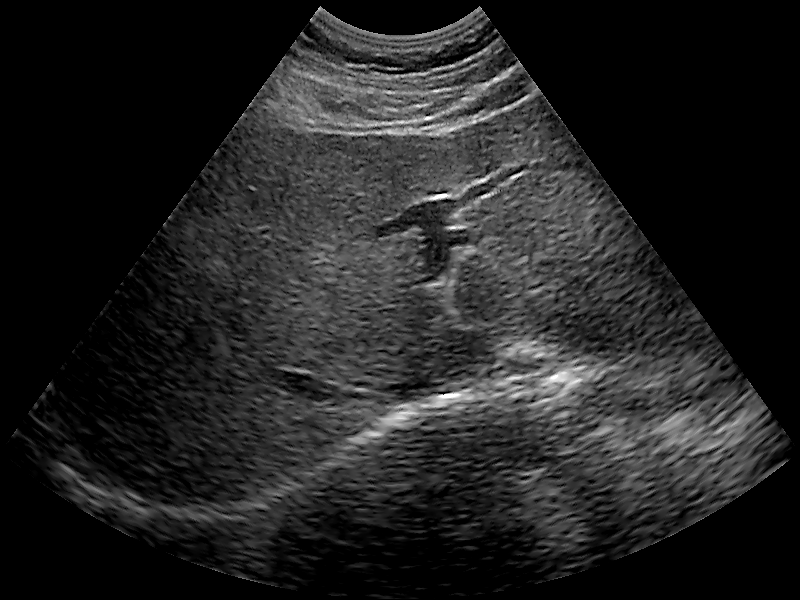
\includegraphics[width=\textwidth, trim={4cm 4cm 4cm 0cm}, clip]{figures/liver1_clpdc.png}};
      \spy on (0.15, 0.0) in node [redwindow, anchor=north] at ($(figA.south)$);
    \end{tikzpicture}
    \caption{CLPD-C}
  \end{subfigure}%
  \begin{subfigure}[b]{0.15\textwidth}
    \begin{tikzpicture}[
        spy using outlines={%
          rectangle,magnification=3,size=\textwidth,
          every spy on node/.append style={transparentwindow}
        }
      ]
      \node (figA) at (0.0,0.0) {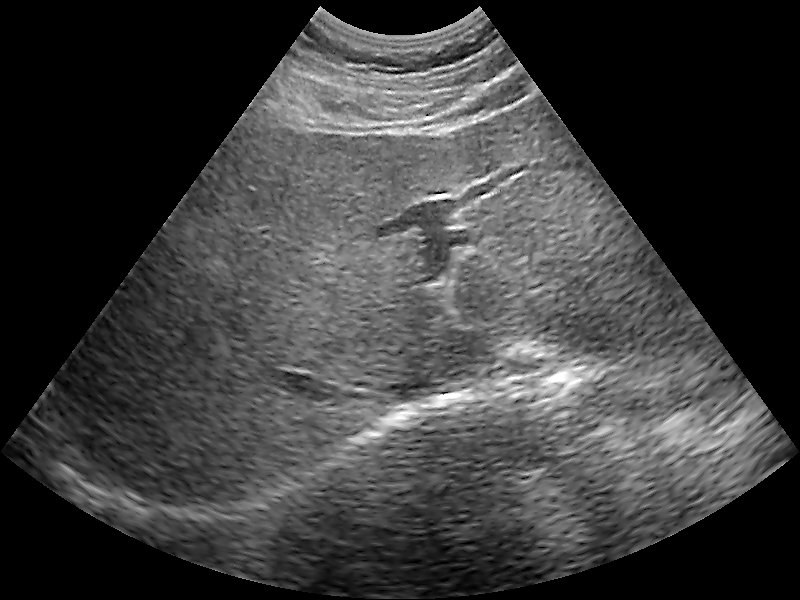
\includegraphics[width=\textwidth, trim={4cm 4cm 4cm 0cm}, clip]{figures/liver1_clpdd.png}};
      \spy on (0.15, 0.0) in node [redwindow, anchor=north] at ($(figA.south)$);
    \end{tikzpicture}
    \caption{CLPD-D}
  \end{subfigure}%
  \begin{subfigure}[b]{0.15\textwidth}
    \begin{tikzpicture}[
        spy using outlines={%
          rectangle,magnification=3,size=\textwidth,
          every spy on node/.append style={redwindow}
        }
      ]
      \node (figA) at (0.0,0.0) {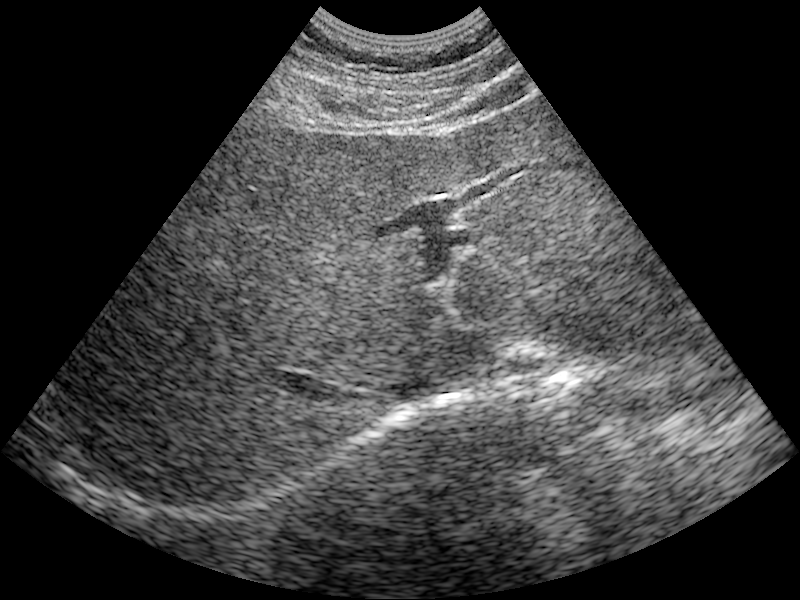
\includegraphics[width=\textwidth, trim={4cm 4cm 4cm 0cm}, clip]{figures/liver1.png}};
      \spy on (0.15, 0.0) in node [redwindow, anchor=north] at ($(figA.south)$);
    \end{tikzpicture}
    \caption{Original}\label{fig:liver_original}
  \end{subfigure}
  \caption{Results on liver image.}\label{fig:liver1}
\end{figure*}

%%% Local Variables:
%%% TeX-master: "master"
%%% End:
